\chapter{End-to-End Machine Learning Project\label{End-to-End Machine Learning Project}}
\section{Working with Real Data\label{Working with Real Data}}

When you are learning about Machine Learning, it is best to experiment with realworld data, not artificial datasets. Here are a few places you can look
to get data:
\begin{itemize}
\item Popular open data repositories
\begin{itemize}
\item \href{http://archive.ics.uci.edu/ml/index.php}{UC Irvine Machine Learning Repository}

\item \href{https://www.kaggle.com/datasets}{Kaggle datasets}

\item \href{https://registry.opendata.aws/}{Amazon's AWS datasets}
\end{itemize}

\item Meta portals (they list open data repositories)
\begin{itemize}
\item \href{http://dataportals.org/}{Data Portals}

\item \href{http://opendatamonitor.eu/}{OpenDataMonitor}

\item \href{https://data.nasdaq.com/}{Quandl}
\end{itemize}

\item Other pages listing many popular open data repositories
\begin{itemize}
\item \href{https://en.wikipedia.org/wiki/List_of_datasets_for_machine-learning_research}{Wikipedia's list of Machine Learning datasets}

\item\href{https://www.quora.com/Where-can-I-find-large-datasets-open-to-the-public}{Quora.com}

\item\href{https://www.reddit.com/r/datasets/}{The datasets subreddit}
\end{itemize}
\end{itemize}

\section{Look at the Big Picture}
\subsection{Frame the Problem}
The first question to ask your boss is what exactly the business objective is. Building a
model is probably not the end goal. How does the company expect to use and benefit
from this model? Knowing the objective is important because it will determine how
you frame the problem, which algorithms you will select, which performance measure you will use to evaluate your model, and how much effort you will spend tweaking it.

Your boss answers that your model's output (a prediction of a district's median housing price) will be fed to another Machine Learning system (see \autoref{A Machine Learning pipeline for real estate investments}), along
with many other signals\footnote{A piece of information fed to a Machine Learning system is often called a signal, in reference to Claude Shannon's information theory, which he developed at Bell Labs to improve telecommunications. His theory: you
want a high signal-to-noise ratio.}.

\begin{figure}
\centering
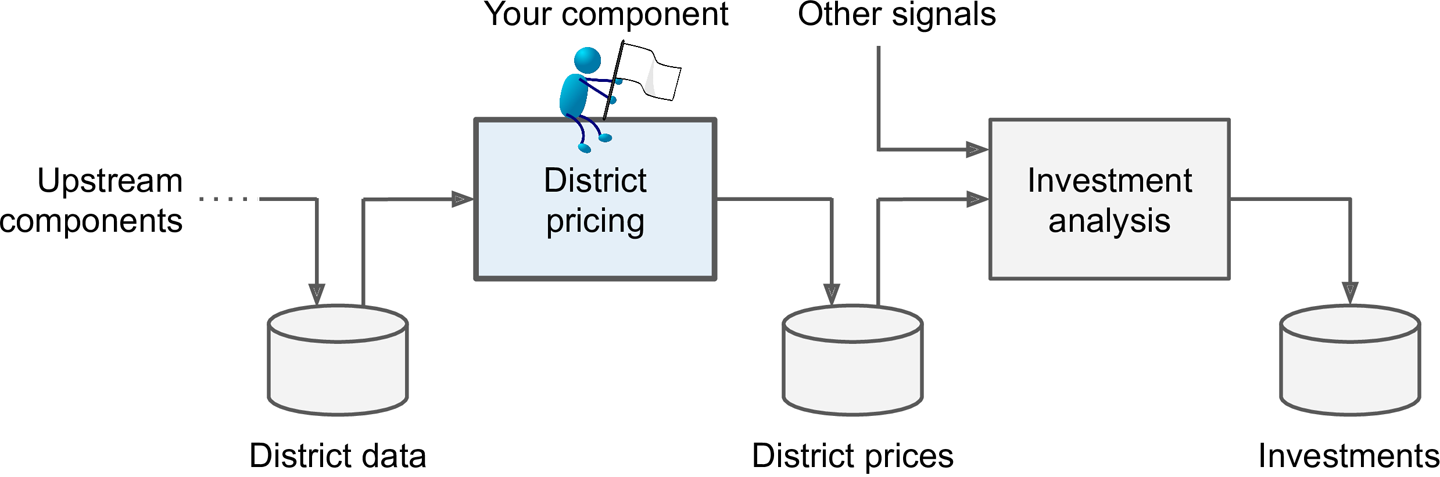
\includegraphics{img/A Machine Learning pipeline for real estate investments.png}
\caption{A Machine Learning pipeline for real estate investments}
\label{A Machine Learning pipeline for real estate investments}
\end{figure}
\explain{Pipelines}{
A sequence of data processing components is called a data pipeline. Pipelines are very
common in Machine Learning systems, since there is a lot of data to manipulate and
many data transformations to apply.

Components typically run asynchronously. Each component pulls in a large amount
of data, processes it, and spits out the result in another data store. Then, some time
later, the next component in the pipeline pulls this data and spits out its own output.
Each component is fairly self-contained: the interface between components is simply
the data store. This makes the system simple to grasp (with the help of a data flow
graph), and different teams can focus on different components. Moreover, if a component breaks down, the downstream components can often continue to run normally (at least for a while) by just using the last output from the broken component.
This makes the architecture quite robust.

On the other hand, a broken component can go unnoticed for some time if proper
monitoring is not implemented. The data gets stale and the overall system's performance drops.
}

The next question to ask your boss is what the current solution looks like (if any).
The current situation will often give you a reference for performance

\textbf{Tips:}If the data were huge, you could either split your batch learning
work across multiple servers (using the MapReduce technique) or
use an online learning technique.

\subsection{Select a Performance Measure}
Your next step is to select a performance measure. A typical performance measure for
regression problems is the Root Mean Square Error (RMSE). It gives an idea of how
much error the system typically makes in its predictions, with a higher weight for
large errors. \autoref{RMSE} shows the mathematical formula to compute the RMSE.

\begin{equation}\label{RMSE}
RMSE(\mathbf{X}, h) = \sqrt{\frac{1}{m}\sum_{i=1}^m(h(x^{(i)})-y^{(i)})^2}
\end{equation}

\explain{Notations}{
This equation introduces several very common Machine Learning notations that we
will use throughout this book:
\begin{itemize}
\item $m$ is the number of instances in the dataset you are measuring the RMSE on.

\item $\mathbf{x}^{(i)}$ is a vector of all the feature values (excluding the label) of the $i^{th}$ instance in
the dataset, and $y^{(i)}$ is its label (the desired output value for that instance). e.g., 
\begin{align*}
\mathbf{x}^{(i)}&=\begin{bmatrix}
-118.29\\
33.91\\
1,416\\
38,372
\end{bmatrix}
\end{align*}


\item
$\mathbf{X}$ is a matrix containing all the feature values (excluding labels) of all instances in
the dataset. There is one row per instance, and the $i^{th}$ row is equal to the transpose of $\mathbf{x}^{(i)}$, noted $(\mathbf{x}^{(i)})^T$. e.g.,

\begin{align*}
\mathbf{x}^{(i)}&=\begin{bmatrix}
(\mathbf{x}^{(1)})^T\\
(\mathbf{x}^{(2)})^T\\
\vdots\\
(\mathbf{x}^{(m-1)})^T\\
(\mathbf{x}^{(m)})^T
\end{bmatrix}=\begin{bmatrix}
-118.29&33.91&1,416&38,372\\
\vdots&\vdots&\vdots&\vdots\\
\end{bmatrix}
\end{align*}
\item  $h$ is your system's prediction function, also called a \emph{hypothesis}. When your system
is given an instance's feature vector $\mathbf{x}^{(i)}$, it outputs a predicted value $\hat{y}^{(i)} = h(\mathbf{x}^{(i)})$ for that instance.

\item $RMSE(\mathbf{X}, h)$ is the cost function measured on the set of examples using your
hypothesis \emph{h}.

We use lowercase italic font for scalar values and function names, lowercase bold font for vectors, and uppercase bold font for
matrices.
\end{itemize}
}

Even though the RMSE is generally the preferred performance measure for regression
tasks, in some contexts you may prefer to use another function. For example, \textbf{suppose
that there are many outlier districts. In that case, you may consider using the mean
absolute error} (MAE, also called the average absolute deviation; see \autoref{MAE}):

\begin{equation}\label{MAE}
MAE(\mathbf{X}, h) = \frac{1}{m}\sum_{i=1}^m|h(x^{(i)})-y^{(i)}|
\end{equation}

Both the RMSE and the MAE are ways to measure the distance between two vectors:
the vector of predictions and the vector of target values. Various distance measures,
or \emph{norms}, are possible:

\begin{itemize}
\item
Computing the root of a sum of squares (RMSE) corresponds to the \emph{Euclidean
norm}: this is the notion of distance you are familiar with. It is also called the \emph{$l_2$
norm}, noted $||\cdot||_2$ (or just$||\cdot||$).
\item
Computing the sum of absolutes (MAE) corresponds to the \emph{$l_1$ norm}, noted $||\cdot||_1$.
This is sometimes called the \emph{Manhattan norm} because it measures the distance
between two points in a city if you can only travel along orthogonal city blocks.
\item More generally, the $l_k$ norm of a vector $v$ containing $n$ elements is defined as $||v||_k
= (|v_0|^k + |v_1|^k + \cdots + |v_n|^k)^{1/k}$. $l_0$ gives the number of nonzero elements in the vector, and $l_\infty$ gives the maximum absolute value in the vector.
\item \textbf{The higher the norm index, the more it focuses on large values and neglects small
ones.} This is why the RMSE is more sensitive to outliers than the MAE. But when
outliers are exponentially rare (like in a bell-shaped curve), the RMSE performs
very well and is generally preferred.
\end{itemize}

\subsection{Check the Assumptions}
Lastly, it is good practice to list and verify the assumptions that have been made so far
(by you or others); this can help you catch serious issues early on. For example, the
district prices that your system outputs are going to be fed into a downstream
Machine Learning system, and you assume that these prices are going to be used as
such. But what if the downstream system converts the prices into categories (e.g.,
``cheap,” ``medium,” or ``expensive”) and then uses those categories instead of the pri‐
ces themselves? In this case, getting the price perfectly right is not important at all;
your system just needs to get the category right. If that's so, then the problem should
have been framed as a classification task, not a regression task. You don't want to find
this out after working on a regression system for months.

\section{Get the Data}
The full Jupyter notebook is available at \url{https://github.com/JPL-JUNO/HOML}.
\subsection{Create the Workspace}
You will need to have Python installed. It is probably already installed on your
system. If not, you can get it at \url{https://www.python.org/}.

If you already have Jupyter running with all these modules installed,
you can safely skip to \nameref{Download the Data}.
\subsection{Download the Data\label{Download the Data}}

Having a function that downloads the data is useful in particular if the
data changes regularly: you can write a small script that uses the function to fetch the
latest data (or you can set up a scheduled job to do that automatically at regular intervals). Automating the process of fetching the data is also useful if you need to install
the dataset on multiple machines.

\subsection{Take a Quick Look at the Data Structure}
Let's take a look at the five rows using the DataFrame's \verb|sample(n=5)| method instead of \verb|head(n=5)|.

The \verb|info()| method is useful to get a quick description of the data, in particular the
total number of rows, each attribute's type, and the number of nonnull values. Notice that the 
\verb|total_bedrooms| attribute has only 20,433 nonnull values, meaning that 207 districts are missing
this feature. We will need to take care of this later.

You can find out what cate‐
gories exist and how many districts belong to each category by using the
\verb|value_counts()| method:

\begin{minted}{python}
housing['ocean_proximity'].value_counts()
\end{minted}

The \verb|describe()| method shows a summary of the
numerical attributes. When with many columns, you can use \verb|transpose()| for best information.
\begin{minted}{python}
# housing.describe()
housing.describe().transpose()
\end{minted}

Another quick way to get a feel of the type of data you are dealing with is to plot a
histogram for each numerical attribute. A histogram shows the number of instances
(on the vertical axis) that have a given value range (on the horizontal axis). You can
either plot this one attribute at a time, or you can call the \verb|hist()| method on the whole dataset, and it will plot a histogram
for each numerical attribute (see \autoref{A histogram for each numerical attribute}):
\begin{minted}{python}
%matplotlib inline
import matplotlib.pyplot as plt
housing.hist(bins=50, figsize=(20, 15))
plt.show()
\end{minted}

\begin{pyc}
%matplotlib inline
import matplotlib.pyplot as plt
housing.hist(bins=50, figsize=(20, 15))
plt.show()
\end{pyc}

\begin{figure}
\centering
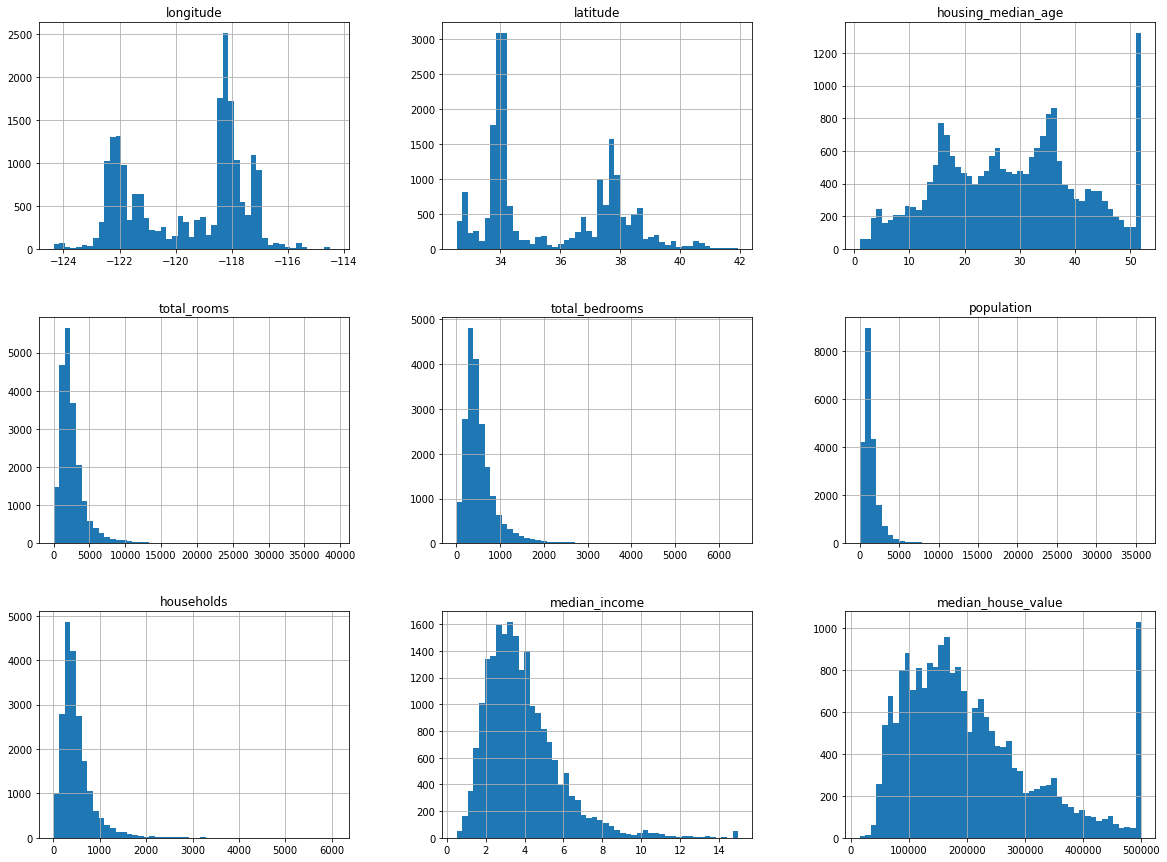
\includegraphics{img/codes/A histogram for each numerical attribute.png}
\caption{A histogram for each numerical attribute}
\label{A histogram for each numerical attribute}
\end{figure}

\notes{
The \texttt{hist()} method relies on Matplotlib, which in turn relies on a
user-specified graphical backend to draw on your screen. So before
you can plot anything, you need to specify which backend Matplotlib should use. The simplest option is to use Jupyter's magic command \texttt{\%matplotlib inline}. This tells Jupyter to set up Matplotlib
so it uses Jupyter's own backend. Plots are then rendered within the
notebook itself. Note that calling \texttt{show()} is optional in a Jupyter
notebook, as Jupyter will automatically display plots when a cell is
executed.
}

There are a few things you might notice in these histograms:
\begin{enumerate}
\item First, the median income attribute does not look like it is expressed in US dollars
(USD). After checking with the team that collected the data, you are told that the
data has been scaled and capped at 15 (actually, 15.0001) for higher median
incomes, and at 0.5 (actually, 0.4999) for lower median incomes. Working with preprocessed attributes is common in Machine Learning, and it is not necessarily a problem, but you should try to understand how the
data was computed.
\item
The housing median age and the median house value were also capped. The latter may be a serious problem since it is your target attribute (your labels). Your
Machine Learning algorithms may learn that prices never go beyond that limit.
You need to check with your client team (the team that will use your system's output) to see if this is a problem or not. If they tell you that they need precise predictions even beyond \$500,000, then you have two options:
\begin{enumerate}
\item Collect proper labels for the districts whose labels were capped.
\item Remove those districts from the training set (and also from the test set, since
your system should not be evaluated poorly if it predicts values beyond
\$500,000).
\end{enumerate} 
\item These attributes have very different scales. We will discuss this later in this chapter, when we explore feature scaling.

\item Finally, many histograms are \emph{tail-heavy}: they extend much farther to the right of
the median than to the left. This may make it a bit harder for some Machine
Learning algorithms to detect patterns. We will try transforming these attributes
later on to have more bell-shaped distributions.
\end{enumerate}

\warning{Wait! Before you look at the data any further, you need to create a
test set, put it aside, and never look at it.}

\subsection{Create a Test Set}
It may sound strange to voluntarily set aside part of the data at this stage. After all,
you have only taken a quick glance at the data, and surely you should learn a whole
lot more about it before you decide what algorithms to use, right? This is true, but
your brain is an amazing pattern detection system, which means that it is highly
prone to overfitting: if you look at the test set, you may stumble upon some seemingly
interesting pattern in the test data that leads you to select a particular kind of
Machine Learning model. When you estimate the generalization error using the test
set, your estimate will be too optimistic, and you will launch a system that will not
perform as well as expected. This is called \emph{data snooping} bias.

Creating a test set is theoretically simple: pick some instances randomly, typically
20\% of the dataset (or less if your dataset is very large), and set them aside:
\begin{pyc}
import numpy as np
def split_train_test(data, test_ratio):
    shuffled_indices = np.random.permutation(len(data))
    test_set_size = int(len(data) * test_ratio)
    test_indices = shuffled_indices[: test_set_size]
    train_indices = shuffled_indices[test_set_size: ]
    return data.iloc[train_indices], data.iloc[test_indices]

train_set, test_set = split_train_test(housing, .2)
len(train_set), len(test_set)
# (16512, 4128)
\end{pyc}

Well, this works, but it is not perfect: if you run the program again, it will generate a different test set! Over time, you (or your Machine Learning algorithms) will get to
see the whole dataset, which is what you want to avoid.

One solution is to save the test set on the first run and then load it in subsequent
runs. \textbf{Another option is to set the random number generator's seed} (e.g., with \verb|np.random.seed(42)|)\footnote{You will often see people set the random seed to 42. This number has no special property, other than to be the
Answer to the Ultimate Question of Life, the Universe, and Everything.} before calling \verb|np.random.permutation()| so that it always generates
the same shuffled indices.

But both these solutions will break the next time you fetch an updated dataset. To
have a stable train/test split even after updating the dataset, a common solution is to
use each instance's identifier to decide whether or not it should go in the test set
(assuming instances have a unique and immutable identifier). For example, you could
compute a hash of each instance's identifier and put that instance in the test set if the
hash is lower than or equal to 20\% of the maximum hash value. This ensures that the
test set will remain consistent across multiple runs, even if you refresh the dataset.
The new test set will contain 20\% of the new instances, but it will not contain any
instance that was previously in the training set.

Here is a possible implementation(more about \href{https://baike.baidu.com/item/CRC32/7460858}{crc32}):
\begin{pyc}
from zlib import crc32
def test_set_check(identifier, test_ratio):
    return crc32(np.int64(identifier)) & 0xffffffff < test_ratio * 2 ** 32

def split_train_test_by_id(data, test_ratio, id_column):
    ids = data[id_column]
    in_test_set = ids.apply(lambda id_: test_set_check(id_, test_ratio))
    return data.loc[~in_test_set], data.loc[in_test_set]

housing_with_id = housing.reset_index()
train_set, test_set = split_train_test_by_id(housing_with_id, .2, 'index')
len(train_set), len(test_set)
# (16512, 4128)
\end{pyc}

If you use the row index as a unique identifier, you need to make sure that new data
gets appended to the end of the dataset and that no row ever gets deleted. If this is not
possible, then \textbf{you can try to use the most stable features to build a unique identifier}. For example, a district's latitude and longitude are guaranteed to be stable for a few
million years, so you could combine them into an ID like so:

\begin{pyc}
housing_with_id['id'] = housing['longitude'] * 1000 + housing['latitude']
train_set, test_set = split_train_test_by_id(housing_with_id, .2, 'id')
len(train_set), len(test_set)
# (16322, 4318)
\end{pyc}

Scikit-Learn provides a few functions to split datasets into multiple subsets in various
ways. The simplest function is \verb|train_test_split()|. First, there is a \verb|random_state| parameter that allows you to set the random generator
seed. Second, you can pass it multiple datasets with an identical number of rows, and
it will split them on the same indices (this is very useful, for example, if you have a
separate DataFrame for labels):
\begin{pyc}
from sklearn.model_selection import train_test_split
train_set, test_set = train_test_split(housing, test_size=.2, random_state=42)
len(train_set), len(test_set)
# (16512, 4128)
\end{pyc}

So far we have considered purely random sampling methods. This is generally fine if
your dataset is large enough (especially relative to the number of attributes), but if it
is not, you \textbf{run the risk of introducing a significant sampling bias}. When a survey
company decides to call 1,000 people to ask them a few questions, they don't just pick
1,000 people randomly in a phone book. They try to ensure that these 1,000 people
are representative of the whole population. For example, the US population is 51.3\%
females and 48.7\% males, so a well-conducted survey in the US would try to maintain
this ratio in the sample: 513 female and 487 male. This is called stratified sampling:
the population is divided into homogeneous subgroups called strata, and the right
number of instances are sampled from each stratum to guarantee that the test set is
representative of the overall population. If the people running the survey used purely
random sampling, there would be about a 11.29\% chance of sampling a skewed test set that was either less than 49\% female or more than 54\% female(Why see \href{https://github.com/JPL-JUNO/HOML/blob/main/chapter/chapter2.ipynb}{Notebook chapter2}). Either way, the survey results would be significantly biased.

Suppose you chatted with experts who told you that the median income is a very
important attribute to predict median housing prices. You may want to ensure that
the test set is representative of the various categories of incomes in the whole dataset. It is important to have a sufficient number of instances in your dataset for each stratum, or else the estimate
of a stratum's importance may be biased. \textbf{This means that you should not have too
many strata, and each stratum should be large enough.}

\begin{pyc}
housing['income_cat'] = pd.cut(housing['median_income'],
                               bins=[0, 1.5, 3.0, 4.5, 6, np.inf], 
                               labels=[1, 2, 3, 4, 5])
housing['income_cat'].hist()
\end{pyc}
\begin{figure}
\centering
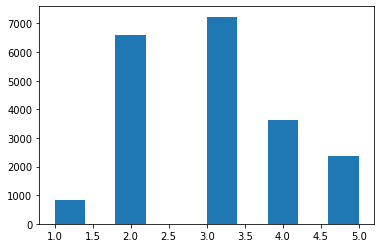
\includegraphics{img/codes/Histogram of income categories.png}
\caption{Histogram of income categories}
\label{Histogram of income categories}
\end{figure}
Now you are ready to do stratified sampling based on the income category. For this
you can use Scikit-Learn's \verb|StratifiedShuffleSplit|(more about \href{https://scikit-learn.org/stable/modules/cross_validation.html}{StratifiedShuffleSplit}) class:

\begin{pyc}
from sklearn.model_selection import StratifiedShuffleSplit
split = StratifiedShuffleSplit(n_splits=1, test_size=.2, random_state=42)
for train_index, test_index in split.split(housing, housing['income_cat']):
    strat_train_set = housing.loc[train_index]
    strat_test_set = housing.loc[test_index]
strat_test_set['income_cat'].value_counts() / len(strat_test_set)
\end{pyc}

 As you can see, the test set generated using stratified sampling has
income category proportions almost identical to those in the full dataset, whereas the
test set generated using purely random sampling is skewed(for more see \href{https://github.com/JPL-JUNO/HOML/blob/main/chapter/chapter2.ipynb}{Notebook chapter2}).

Now you should remove the \verb|income_cat| attribute so the data is back to its original
state:
\begin{pyc}
for set_ in (strat_train_set, strat_test_set):
    set_.drop('income_cat', axis='columns', inplace=True)
\end{pyc}

We spent quite a bit of time on test set generation for a good reason: this is an often
neglected but critical part of a Machine Learning project. Moreover, many of these
ideas will be useful later when we discuss cross-validation.

\section{Discover and Visualize the Data to Gain Insights}
First, make sure you have put the test set aside and you are only exploring the training set. Also, if the training set is very large, you may want to sample an exploration
set, to make manipulations easy and fast.

\subsection{Visualizing Geographical Data}

Since there is geographical information (latitude and longitude), it is a good idea to
create a scatterplot of all districts to visualize the data (\autoref{A geographical scatterplot of the data}):
\figures{A geographical scatterplot of the data}

Setting the alpha option to 0.1 makes it much easier to visualize the places
where there is a high density of data points(\autoref{A better visualization that highlights high-density areas}).

\figures{A better visualization that highlights high-density areas}

Our brains are very good at spotting patterns in pictures, but you may need to play
around with visualization parameters to make the patterns stand out.

Now let's look at the housing prices (\autoref{California housing prices}).
\figures{California housing prices}
\begin{pyc}
housing.plot(kind='scatter', x='longitude', y='latitude', alpha=.4, s=housing['population']/100,
             label='population', figsize=(10, 7),
             c='median_house_value', cmap=plt.get_cmap('jet'), colorbar=True)
plt.legend()
plt.show()
\end{pyc}


This image tells you that the housing prices are very much related to the location
(e.g., close to the ocean) and to the population density, as you probably knew already.
A clustering algorithm should be useful for detecting the main cluster and for adding
new features that measure the proximity to the cluster centers. The ocean proximity
attribute may be useful as well, although in Northern California the housing prices in
coastal districts are not too high, so it is not a simple rule.

\subsection{Looking for Correlations}
Since the dataset is not too large, you can easily compute the \emph{standard correlation
coefficient} (also called \emph{Pearson's r}) between every pair of attributes using the \verb|corr()| method:
\begin{pyc}
corr_matrix = housing.corr()
corr_matrix['median_house_value'].sort_values(ascending=False)
\end{pyc}

\autoref{Standard correlation coefficient of various datasets} shows various plots along with the correlation coefficient between their horizontal and vertical axes.

\figures{Standard correlation coefficient of various datasets}
\warning{The correlation coefficient only measures linear correlations (``if x
goes up, then y generally goes up/down”). It may completely miss
out on nonlinear relationships (e.g., ``if x is close to 0, then y generally goes up”). }

Another way to check for correlation between attributes is to use the pandas
\verb|scatter_matrix()| function, which plots every numerical attribute against every other numerical attribute(\href{https://github.com/JPL-JUNO/HOML/blob/main/chapter/chapter2.ipynb}{You can see here}).

The most promising attribute to predict the median house value is the median
income, so let's zoom in on their correlation scatterplot (\autoref{Median income versus median house value}):

\figures{Median income versus median house value}

This plot reveals a few things. First, the correlation is indeed very strong; you can
clearly see the upward trend, and the points are not too dispersed. Second, the price
cap that we noticed earlier is clearly visible as a horizontal line at \$500,000. But this
plot reveals other less obvious straight lines: a horizontal line around \$450,000,
another around \$350,000, perhaps one around \$280,000, and a few more below that.
You may want to try removing the corresponding districts to prevent your algorithms
from learning to reproduce these data quirks.

\subsection{Experimenting with Attribute Combinations}

\subsection{Handling Text and Categorical Attributes}
Most Machine Learning algorithms prefer to work with numbers, so let's convert these categories from
text to numbers. For this, we can use Scikit-Learn's OrdinalEncoder class:

\begin{pyc}
from sklearn.preprocessing import OrdinalEncoder
ordinal_encoder = OrdinalEncoder()
housing_cat_encoded = ordinal_encoder.fit_transform(housing_cat)
housing_cat_encoded[:10]
\end{pyc}
You can get the list of categories using the \verb|categories_| instance variable. It is a list
containing a 1D array of categories for each categorical attribute (in this case, a list
containing a single array since there is just one categorical attribute):

One issue with this representation is that ML algorithms will assume that two nearby values are more similar than two distant values. This may be fine in some cases (e.g., for ordered categories such as ``bad,” ``average,” ``good,” and ``excellent”), but it is obviously not the case for the \verb|ocean_proximity| column (for example, categories 0 and 4 are clearly more similar than categories 0 and 1). To fix this issue, a common solution is to create one binary attribute per category: one attribute equal to 1 when the category is ``$\textless$1H OCEAN” (and 0 otherwise), another attribute equal to 1 when the category is ``INLAND” (and 0 otherwise), and so on. This is called one-hot encoding,
because only one attribute will be equal to 1 (hot), while the others will be 0 (cold).
The new attributes are sometimes called dummy attributes. Scikit-Learn provides a
OneHotEncoder class to convert categorical values into one-hot vectors:

\begin{pyc}
from sklearn.preprocessing import OneHotEncoder
cat_encoder = OneHotEncoder()
housing_cat_1hot = cat_encoder.fit_transform(housing_cat)
housing_cat_1hot
\end{pyc}

Notice that the output is a SciPy \emph{sparse matrix}, instead of a NumPy array. This is very
useful when you have categorical attributes with thousands of categories. After one-hot encoding, we get a matrix with thousands of columns, and the matrix is full of 0s
except for a single 1 per row. Using up tons of memory mostly to store zeros would
be very wasteful, so instead a sparse matrix only stores the location of the nonzero
elements. You can use it mostly like a normal 2D array but if you really want to convert it to a (dense) NumPy array, just call the \verb|toarray()| method.

\tips{If a categorical attribute has a large number of possible categories
(e.g., country code, profession, species), then one-hot encoding will
result in a large number of input features. This may slow down
training and degrade performance. If this happens, you may want
to replace the categorical input with useful numerical features
related to the categories: for example, you could replace the
ocean\_proximity feature with the distance to the ocean (similarly,
a country code could be replaced with the country's population and
GDP per capita). Alternatively, you could replace each category
with a learnable, low-dimensional vector called an embedding. Each
category's representation would be learned during training. This is
an example of representation learning (see Chapters \autoref{13} and \autoref{17} for
more details).}

\subsection{Feature Scaling and Transformation}
One of the most important transformations you need to apply to your data is \emph{feature scaling}. With few exceptions, machine learning algorithms don't perform well when the input numerical attributes have very different scales. There are two common ways to get all attributes to have the same scale: \emph{min-max scaling} and \emph{standardization}.

\warning{As with all estimators, it is important to fit the scalers to the training data only: never use fit() or fit\_transform() for anything else than the training set. Once you have a trained scaler, you can then use it to transform() any other set, including the validation set, the test set, and new data. Note that while the training set values will always be scaled to the specified range, if new data contains outliers, these may end up scaled outside the range. If you want to avoid this, just set the clip hyperparameter to True.}

Min-max scaling (many people call this normalization) is the simplest: for each
attribute, the values are shifted and rescaled so that they end up ranging from
0 to 1. This is performed by subtracting the min value and dividing by the difference between the min and the max. Scikit-Learn provides a transformer called
MinMaxScaler for this. It has a \verb|feature_range| hyperparameter that lets you change
the range if, for some reason, you don't want 0–1 (e.g., neural networks work best
with zero-mean inputs, so a range of –1 to 1 is preferable).

Standardization is different: first it subtracts the mean value (so standardized values
have a zero mean), then it divides the result by the standard deviation (so standardized values have a standard deviation equal to 1). Unlike min-max scaling, standardization does not restrict values to a specific range. However, standardization is much
less affected by outliers. For example, suppose a district has a median income equal to 100 (by mistake), instead of the usual 0–15. Min-max scaling to the 0–1 range would map this outlier down to 1 and it would crush all the other values down to 0–0.15, whereas standardization would not be much affected. Scikit-Learn provides a transformer called StandardScaler for standardization.

\tips{If you want to scale a sparse matrix without converting it to a dense matrix first, you can use a StandardScaler with its with\_mean hyperparameter set to False: it will only divide the data by the standard deviation, without subtracting the mean (as this would break sparsity).}

When a feature's distribution has a heavy tail (i.e., when values far from the mean are not exponentially rare), both min-max scaling and standardization will squash most values into a small range. Machine learning models generally don't like this at all, as you will see in \autoref{Training Models}. So \textbf{before you scale the feature, you should first transform it to shrink the heavy tail, and if possible to make the distribution roughly symmetrical}. For example, a common way to do this for positive features with a heavy tail to the right is to replace the feature with its square root (or raise the feature to a power between 0 and 1). If the feature has a really long and heavy tail, such as a power law distribution, then replacing the feature with its logarithm may help. For example, the population feature roughly follows a power law: districts with 10,000 inhabitants are only 10 times less frequent than districts with 1,000 inhabitants, not exponentially less frequent. \autoref{Transforming a feature to make it closer to a Gaussian distribution} shows how much better this feature looks when you compute its log: it's very close to a Gaussian distribution (i.e., bell-shaped).

\figures{Transforming a feature to make it closer to a Gaussian distribution}

Another approach to handle heavy-tailed features consists in \emph{bucketizing} the feature.
(对数据进行分箱处理)。 This means chopping its distribution into roughly equal-sized buckets, and replacing each feature value with the index of the bucket it belongs to.

When a feature has a multimodal distribution (i.e., with two or more clear peaks, called modes), it can also be helpful to bucketize it, but this time treating the bucket IDs as categories, rather than as numerical values. 

Another approach to transforming multimodal distributions is to add a feature for
each of the modes (at least the main ones), representing the similarity between the
data and that particular mode. The similarity measure is typically
computed using a \emph{radial basis function (RBF, 径向基函数)}---any function that depends only on the distance between the input value and a fixed point. The most commonly used RBF is
the Gaussian RBF, whose output value decays exponentially as the input value moves
away from the fixed point. \autoref{Gaussian RBF feature measuring the similarity} shows this new feature as a function of the housing median age (solid
line).

\figures{Gaussian RBF feature measuring the similarity}

So far we've only looked at the input features, but the target values may also need
to be transformed. For example, if the target distribution has a heavy tail, you may
choose to replace the target with its logarithm. 

Luckily, most of Scikit-Learn's transformers have an \verb|inverse_transform()| method,
making it easy to compute the inverse of their transformations.

\begin{pyc}
from sklearn.linear_model import LinearRegression

target_scalar = StandardScaler()
scaled_labels = target_scalar.fit_transform(housing_labels.to_frame())

model = LinearRegression()
model.fit(housing[['median_income']], scaled_labels)
# pretend this is new data
some_new_data = housing[['median_income']].iloc[:5]

scaled_predictions = model.predict(some_new_data)
predictions = target_scalar.inverse_transform(scaled_predictions)
# predictions.flatten()
\end{pyc}

This works fine, but a simpler option is to use a \verb|TransformedTargetRegressor|. We
just need to construct it, giving it the regression model and the label transformer,
then fit it on the training set, using the original unscaled labels. It will automatically
use the transformer to scale the labels and train the regression model on the resulting
scaled labels. Then, when we want to make a prediction, it
will call the regression model's \verb|predict()| method and use the scaler's \verb|inverse_transform()| method to produce the prediction.

\begin{pyc}
from sklearn.compose import TransformedTargetRegressor

model = TransformedTargetRegressor(LinearRegression(),
                                    transformer=StandardScaler())
model.fit(housing[['median_income']], housing_labels)
predictions = model.predict(some_new_data)
\end{pyc}
\subsection{Custom Transformers}
Although Scikit-Learn provides many useful transformers, you will need to write
your own for tasks such as custom transformations, cleanup operations, or combining specific attributes.

For transformations that don't require any training, you can just write a function
that takes a NumPy array as input and outputs the transformed array.

\begin{pyc}
from sklearn.preprocessing import FunctionTransformer

log_transformer = FunctionTransformer(np.log, inverse_func=np.exp)
log_pop = log_transformer.transform(housing[['population']])
\end{pyc}

The \verb|inverse_func| argument is optional. Your transformation function can take hyperparameters as additional arguments. Custom transformers are also useful to combine features.

FunctionTransformer is very handy, but what if you would like your transformer to
be trainable, learning some parameters in the fit() method and using them later
in the transform() method? And you will want your transformer to work seamlessly with Scikit-Learn functionalities (such as pipelines), and since Scikit-Learn relies on duck typing (not inheritance), all you need to do is create a class and implement three methods: \verb|fit()|(returning \verb|self|), \verb|transform()|, and \verb|fit_transform()|.

You can get \verb|fit_transform()| for free by simply adding TransformerMixin as a base
class: the default implementation will just call \verb|fit()| and then \verb|transform()|. If you add BaseEstimator as a base class (and avoid using *args and **kwargs in your
constructor), you will also get two extra methods: \verb|get_params()| and \verb|set_params()|. These will be useful for automatic hyperparameter tuning.

\begin{pyc}
from sklearn.base import BaseEstimator, TransformerMixin
from sklearn.utils.validation import check_array, check_is_fitted

class StandardScaler(BaseEstimator, TransformerMixin):
    def __init__(self, with_mean=True):
        self.with_mean = with_mean
        
    def fit(self, X, y=None):
        X = check_array(X)
        self.mean_ = X.mean(axis='index')
        self.scale_ = X.std(axis='index')
        self.n_features_in_ = X.shape[1]
        return self

    def transform(self, X):
        check_is_fitted(self)
        X = check_array(X)
        assert self.n_features_in_ == X.shape[1]
        if self.with_mean:
            X = X - self.mean_
        return X / self.scale_
\end{pyc}

Here are a few things to note:
\begin{itemize}
    \item The sklearn.utils.validation package contains several functions we can use to validate the inputs.
    \item Scikit-Learn pipelines require the fit() method to have two arguments X and y,
    which is why we need the y=None argument even though we don't use y.
    \item All Scikit-Learn estimators set \verb|n_features_in_| in the fit() method, and they
    ensure that the data passed to transform() or predict() has this number of
    features.
    \item The fit() method must return self.

    \item This implementation is not 100\% complete: all estimators should set
    \verb|feature_names_in_| in the fit() method when they are passed a DataFrame.
    Moreover, all transformers should provide a \verb|get_feature_names_out()| method,
    as well as an \verb|inverse_transform()| method when their transformation can be
    reversed.
\end{itemize}

A custom transformer can (and often does) use other estimators in its implementation.

\figures{Gaussian RBF similarity to the nearest cluster center}

\subsection{Transformation Pipelines}
As you can see, there are many data transformation steps that need to be executed
in the right order. Fortunately, Scikit-Learn provides the Pipeline class to help with
such sequences of transformations.

\begin{pyc}
from sklearn.pipeline import Pipeline
from sklearn.impute import SimpleImputer
from sklearn.preprocessing import StandardScaler
num_pipeline = Pipeline([
    ('impute', SimpleImputer(strategy='median')),
    ('standardize', StandardScaler())
])
\end{pyc}

The Pipeline constructor takes a list of name/estimator pairs (2-tuples) defining a sequence of steps. The names can be anything you like, as long as they are unique and don't contain double underscores (\_\_). The estimators must all be transformers (i.e., they must have a \verb|fit_transform()| method), except for the last one, which can be anything: a transformer, a predictor, or any other type of estimator.

If you don't want to name the transformers, you can use the \verb|make_pipeline()| function instead; it takes transformers as positional arguments and creates a Pipeline using the names of the transformers' classes, in lowercase and without underscores.

\begin{pyc}
from sklearn.pipeline import make_pipeline
num_pipeline = make_pipeline(SimpleImputer(strategy='median'), StandardScaler())
\end{pyc}

If multiple transformers have the same name, an index is appended to their names.

When you call the pipeline's fit() method, it calls \verb|fit_transform()| sequentially on
all the transformers, passing the output of each call as the parameter to the next call
until it reaches the final estimator, for which it just calls the fit() method.

If the last estimator were a predictor instead
of a transformer, then the pipeline would have a predict() method rather than a
transform() method. Calling it would sequentially apply all the transformations to
the data and pass the result to the predictor's predict() method.

\begin{pyc}
housing_num_prepared = num_pipeline.fit_transform(housing_num)
housing_num_prepared[: 2].round(2)
\end{pyc}

It would be more convenient to have a single transformer capable of handling
all columns, applying the appropriate transformations to each column. For this,
you can use a \verb|ColumnTransformer|.  Its constructor requires a list of
triplets (3-tuples), each containing a name (which must be unique and not contain
double underscores), a transformer, and a list of names (or indices) of columns that
the transformer should be applied to.

\begin{pyc}
from sklearn.compose import ColumnTransformer

num_attribs = ['longitude', 'latitude', 'housing_median_age', 'total_rooms',
               'total_bedrooms', 'population', 'households', 'median_income']

cat_attribs = ['ocean_proximity']

cat_pipeline = make_pipeline(
    SimpleImputer(strategy='most_frequent'),
    OneHotEncoder(handle_unknown='ignore')
)

preprocessing = ColumnTransformer([
    ('num', num_pipeline, num_attribs),
    ('cat', cat_pipeline, cat_attribs)
])
\end{pyc}

\tips{Instead of using a transformer, you can specify the string "drop"
if you want the columns to be dropped, or you can specify
"passthrough" if you want the columns to be left untouched. By
default, the remaining columns (i.e., the ones that were not listed)
will be dropped, but you can set the remainder hyperparameter to
any transformer (or to "passthrough") if you want these columns
to be handled differently.}

Since listing all the column names is not very convenient, Scikit-Learn provides
a \verb|make_column_selector()| function that returns a selector function you can use
to automatically select all the features of a given type, such as numerical or categorical. You can pass this selector function to the ColumnTransformer instead of
column names or indices. Moreover, if you don't care about naming the transformers, you can use \verb|make_column_transformer()|, which chooses the names for you,
just like \verb|make_pipeline()| does. 

Once again this returns a NumPy array, but you can get the column names using
\verb|preprocessing.get_feature_names_out()| and wrap the data in a nice DataFrame
as we did before.

\warning{
The OneHotEncoder returns a sparse matrix and the num\_pipeline
returns a dense matrix. When there is such a mix of sparse and
dense matrices, the ColumnTransformer estimates the density of the
final matrix (i.e., the ratio of nonzero cells), and it returns a sparse
matrix if the density is lower than a given threshold (by default,
\texttt{sparse\_threshold=0.3}). In this example, it returns a dense matrix.
}

Let's recap what the pipeline will do and why:
\begin{itemize}
    \item 大多数机器学习算法都不太喜欢缺失值,数值型的变量使用中位数进行impute,分类型变量使用频率最高的进行impute;
    \item 因为大多数机器学习算法只接收数值变量,因此分类变量会被进行one-hot编码;
    \item A few ratio features will be computed and added: \verb|bedrooms_ratio|,
    \verb|rooms_per_house|, and \verb|people_per_house|. Hopefully these will better correlate
    with the median house value, and thereby help the ML models.
    \item A few cluster similarity features will also be added. These will likely be more
    useful to the model than latitude and longitude.
    \item Features with a long tail will be replaced by their logarithm, as most models
    prefer features with roughly uniform or Gaussian distributions.
    
    \item All numerical features will be standardized, as most ML algorithms prefer when
    all features have roughly the same scale. 
\end{itemize}

\begin{pyc}
def column_ratio(X):
    return X[:, [0]] / X[:, [1]]

def ratio_name(function_transformer, feature_names_in):
    return ['ratio']

def ratio_pipeline():
    return make_pipeline(
        SimpleImputer(strategy='median'),
        FunctionTransformer(column_ratio, feature_names_out=ratio_name),
        StandardScaler()
    )
    
log_pipeline = make_pipeline(
    SimpleImputer(strategy='median'),
    FunctionTransformer(np.log, feature_names_out='one-to-one'),
    StandardScaler())

cluster_simil = ClusterSimilarity(n_clusters=10, gamma=1, random_state=42)
default_num_pipeline = make_pipeline(SimpleImputer(strategy='median'),
                                      StandardScaler())

preprocessing = ColumnTransformer([
    ('bedrooms', ratio_pipeline(), ['total_bedrooms', 'total_rooms']),
    ('rooms_per_house', ratio_pipeline(), ['total_rooms', 'households']),
    ('people_per_house', ratio_pipeline(), ['population', 'households']),
    ('log', log_pipeline, ['total_bedrooms', 'total_rooms', 'population', 
                             'households', 'median_income']),
    ('geo', cluster_simil, ['latitude', 'longitude']),
    ('cat', cat_pipeline, make_column_selector(dtype_include=object))
],
                                  remainder=default_num_pipeline)
\end{pyc}

If you run this ColumnTransformer, it performs all the transformations and outputs a
NumPy array with 24 features.
\section{Select and Train a Model}

\subsection{Train and Evaluate on the Training Set}
让我们从最基础的线性模型开始:

\begin{pyc}
from sklearn.linear_model import LinearRegression

lin_reg = make_pipeline(preprocessing, LinearRegression())
lin_reg.fit(housing, housing_labels)
\end{pyc}

\begin{pyc}
housing_prediction = lin_reg.predict(housing)
print(housing_prediction[:5].round(-2))
# -2 = rounded to the nearest hundred
print(housing_labels.iloc[: 5].values)
\end{pyc}

Remember that you chose to use the RMSE as your performance
measure, so you want to measure this regression model's RMSE on the whole training
set using Scikit-Learn's \verb|mean_squared_error()| function, with the squared argument
set to False.

\begin{pyc}
from sklearn.metrics import mean_squared_error
line_rmse = mean_squared_error(housing_labels, 
                               housing_prediction,
                               squared=False)
line_rmse
\end{pyc}

This is better than nothing, but clearly not a great score: the \verb|median_housing_values|
of most districts range between \$120,000 and \$265,000, so a typical prediction error
of \$68,628 is really not very satisfying. This is an example of a model underfitting the
training data. When this happens it can mean that the features do not provide enough
information to make good predictions, or that the model is not powerful enough.
As we saw in the previous chapter, \textbf{the main ways to fix underfitting are to select a
more powerful model, to feed the training algorithm with better features, or to reduce
the constraints on the model}. This model is not regularized, which rules out the last
option. You could try to add more features, but first you want to try a more complex
model to see how it does.

我们决定使用更加复杂的决策树回归模型,这个模型更加强大,具有发现数据中非线性关系的的能力,更多见\autoref{Decision Trees}.

\begin{pyc}
from sklearn.tree import DecisionTreeRegressor

tree_reg = make_pipeline(preprocessing, DecisionTreeRegressor(random_state=42))
tree_reg.fit(housing, housing_labels)

housing_predictions = tree_reg.predict(housing)
tree_rmse = mean_squared_error(
    housing_labels,
    housing_predictions,
    squared=False
)
# 0
\end{pyc}
It is much more likely that the model has badly overfit the data. How can you be sure?
As you saw earlier, you don't want to touch the test set until you are ready to launch a
model you are confident about, \textbf{so you need to use part of the training set for training
and part of it for model validation}.

\subsection{Better Evaluation Using Cross-Validation}
One way to evaluate the decision tree model would be to use the \verb|train_test_split()| function to split the training set into a smaller training set and a validation set, then train your models against the smaller training set and evaluate
them against the validation set. It's a bit of effort, but nothing too difficult, and it
would work fairly well.

A great alternative is to use Scikit-Learn's \emph{k-fold cross-validation} feature.(非常消耗算力)
\begin{pyc}
from sklearn.model_selection import cross_val_score

tree_rmses = -cross_val_score(tree_reg, housing, housing_labels,
                              scoring='neg_root_mean_squared_error',
                              cv=10)
pd.Series(tree_rmses).describe()
\end{pyc}
\warning{
    Scikit-Learn's cross-validation features expect a utility function
(greater is better) rather than a cost function (lower is better), so
the scoring function is actually the opposite of the RMSE. It's a
negative value, so you need to switch the sign of the output to get
the RMSE scores.
}

In fact, it seems to perform almost as poorly as the linear regression model! Notice that cross-validation allows you to get not only an estimate of the performance of your model, but also a measure of how precise this estimate is (i.e., its standard deviation). But cross-validation comes at the cost of training the model several times, so it is not always feasible.

Let's try one last model now: the RandomForestRegressor. As you will see in \autoref{Ensemble Learning and Random Forests}, random forests work by training many decision trees on random subsets of the features, then averaging out their predictions. Such models composed of many other models are called ensembles: they are capable of boosting the performance of the underlying model (in this case, decision trees). 

\begin{pyc}
from sklearn.ensemble import RandomForestRegressor

forest_reg = make_pipeline(preprocessing,
                           RandomForestRegressor(random_state=42))
forest_rmses = - cross_val_score(forest_reg, 
                                 housing, 
                                 housing_labels,
                                 scoring='neg_root_mean_squared_error',
                                 cv=10)
pd.Series(forest_rmses).describe()
\end{pyc}
If you train a RandomForest and measure the RMSE on the training set, you will find roughly 17,474: that's much lower, meaning that there's still quite a lot of overfitting going on.(The training error is much lower than the validation error, which usually means that the model has overfit the training set.) Possible solutions are to simplify the model, constrain it (i.e., regularize it), or get a lot more training data. Before you dive much deeper into random forests, however, you should try out many other models from various categories of machine learning algorithms (e.g., several support vector machines with different kernels, and possibly a neural network), without spending too much time tweaking the hyperparameters. The goal is to shortlist a few (two to five) promising models.(在进行调参之前,应该试试更多的模型,而不是一头扎进调参)

\section{Fine-Tune Your Model}
假设你已经有了一些想要建立的模型清单,你现在需要调整优化参数,来看一下怎么做。
\subsection{Grid Search}
最最不智能的方法就是在参数可行集上慢慢的测试,但这几乎是不可能的。Instead, you can use Scikit-Learn's \verb|GridSearchCV| class to search for you. All you need to do is tell it which hyperparameters you want it to experiment with and what values to try out, and it will use cross-validation to evaluate all the possible combinations of hyperparameter values. 
\begin{pyc}
from sklearn.model_selection import GridSearchCV

full_pipeline = Pipeline([
    ('preprocessing', preprocessing),
    ('random_forest', RandomForestRegressor(random_state=42))
])

param_grid = [
    {'preprocessing__geo__n_clusters': [5, 8, 10],
     'random_forest__max_features': [4, 6, 8]},
    {'preprocessing__geo__n_clusters': [10, 15],
     'random_forest__max_features': [6, 8, 10]},
]

grid_search = GridSearchCV(full_pipeline, param_grid, cv=3,
                           scoring='neg_root_mean_squared_error')
grid_search.fit(housing, housing_labels)
\end{pyc}
Notice that you can refer to any hyperparameter of any estimator in a pipeline,
even if this estimator is nested deep inside several pipelines and column transformers. 

For example, when Scikit-Learn sees ``\verb|preprocessing__geo__n_clusters|", it
splits this string at the double underscores, then it looks for an estimator named
``\verb|preprocessing|" in the pipeline and finds the preprocessing ColumnTransformer.
Next, it looks for a transformer named ``geo" inside this ColumnTransformer and
finds the ClusterSimilarity transformer we used on the latitude and longitude
attributes. Then it finds this transformer's \verb|n_clusters| hyperparameter. Similarly,
\verb|random_forest__max_features| refers to the \verb|max_features| hyperparameter of the
estimator named ``\verb|random_forest|", which is of course the RandomForest model (the
\verb|max_features| hyperparameter will be explained in \autoref{Ensemble Learning and Random Forests} \nameref{Ensemble Learning and Random Forests}).

\tips{
    Wrapping preprocessing steps in a Scikit-Learn pipeline allows you to tune the preprocessing hyperparameters along with the model hyperparameters. This is a good thing since they often interact. For example, perhaps increasing n\_clusters requires increasing max\_features as well. If fitting the pipeline transformers is computationally expensive, you can set the pipeline's memory hyperparameter to the path of a caching directory: when you first fit the pipeline, Scikit-Learn will save the fitted transformers to this directory. If you then fit the pipeline again with the same hyperparameters, Scikit-Learn will just load the cached transformers.
}

整个网格搜索会在两个字典指定的参数上共训练15($3\times 3$和$2\times 3$)次,每次进行3次交叉验证。The best model is obtained by setting \verb|n_clusters| to 15 and setting \verb|max_features| to 6. 但是需要注意的是\verb|n_clusters|达到了指定的最大值,你可能需要尝试更大的以获取更好的模型性能

\begin{pyc}
grid_search.best_params_
\end{pyc}

You can access the best estimator using \verb|grid_search.best_estimator_|. If
\verb|GridSearchCV| is initialized with \verb|refit=True| (which is the default), then once it finds
the best estimator using cross-validation, it retrains it on the whole training set. This
is usually a good idea, since feeding it more data will likely improve its performance.

The evaluation scores are available using \verb|grid_search.cv_results_|, which is a dictionary.

\begin{pyc}
cv_res = pd.DataFrame(grid_search.cv_results_)
cv_res.sort_values(by='mean_test_score', ascending=False, inplace=True)
cv_res = cv_res[['param_preprocessing__geo__n_clusters',
                 'param_random_forest__max_features',
                 'split0_test_score',
                 'split1_test_score',
                 'split2_test_score',
                 'mean_test_score']]
score_cols = ['split0', 'split1', 'split2', 'mean_test_rmse']
cv_res.columns = ['n_clusters', 'max_features'] + score_cols
cv_res[score_cols] = - cv_res[score_cols].round().astype(np.int64)
cv_res.head()
\end{pyc}

\subsection{Randomized Search}
The grid search approach is fine when you are exploring relatively few combinations,
like in the previous example, but \verb|RandomizedSearchCV| is often preferable, especially
when the hyperparameter search space is large. This class can be used in much
the same way as the GridSearchCV class, but instead of trying out all possible combinations it evaluates a fixed number of combinations, selecting a random value
for each hyperparameter at every iteration. This may sound surprising, but this
approach has several benefits:
\begin{itemize}
    \item If some of your hyperparameters are continuous (or discrete but with many
    possible values), and you let randomized search run for, say, 1,000 iterations, then
    it will explore 1,000 different values for each of these hyperparameters, whereas
    grid search would only explore the few values you listed for each one.
    \item Suppose a hyperparameter does not actually make much difference, but you don't
    know it yet. If it has 10 possible values and you add it to your grid search, then
    training will take 10 times longer. But if you add it to a random search, it will not
    make any difference.(这个理由我似乎不太明白在讲什么)
    \item If there are 6 hyperparameters to explore, each with 10 possible values, then grid
    search offers no other choice than training the model a million times, whereas
    random search can always run for any number of iterations you choose.
\end{itemize}

\begin{pyc}
from sklearn.model_selection import RandomizedSearchCV
from scipy.stats import randint

param_distribs = {
    'preprocessing__geo__n_clusters': randint(low=3, high=50),
    'random_forest__max_features': randint(low=2, high=20)
}

rnd_search = RandomizedSearchCV(
    full_pipeline, param_distributions=param_distribs, n_iter=10, cv=3,
    scoring='neg_root_mean_squared_error', random_state=42
)

rnd_search.fit(housing, housing_labels)
\end{pyc}

Scikit-Learn also has \verb|HalvingRandomSearchCV| and \verb|HalvingGridSearchCV| hyperparameter search classes. Their goal is to use the computational resources more efficiently,
either to train faster or to explore a larger hyperparameter space. Here's how they
work: in the first round, many hyperparameter combinations (called ``candidates”) are
generated using either the grid approach or the random approach. These candidates
are then used to train models that are evaluated using cross-validation, as usual.
However, training uses limited resources, which speeds up this first round considerably. By default, ``limited resources” means that the models are trained on a small
part of the training set. However, other limitations are possible, such as reducing
the number of training iterations if the model has a hyperparameter to set it. Once
every candidate has been evaluated, only the best ones go on to the second round,
where they are allowed more resources to compete. After several rounds, the final
candidates are evaluated using full resources. This may save you some time tuning
hyperparameters.

在随机网格中,如何去选择超参数的采样分布?

\begin{itemize}
    \item \verb|scipy.stats.randint(a, b+1)|(\href{https://docs.scipy.org/doc/scipy/reference/generated/scipy.stats.randint.html}{随机整数}): for hyperparameters with discrete values that range from a to b, and all values in that range seem equally likely.
    \item \verb|scipy.stats.uniform(a, b)|(\href{https://docs.scipy.org/doc/scipy/reference/generated/scipy.stats.uniform.html}{均匀分布}): this is very similar, but for continuous hyperparameters.
    \item \verb|scipy.stats.geom(1 / scale)|(\href{https://docs.scipy.org/doc/scipy/reference/generated/scipy.stats.geom.html}{几何分布}): for discrete values, when you want to sample roughly in a given scale. E.g., with scale=1000 most samples will be in this ballpark, but about 10\% of all samples will be $\textless 100$ and about 10\% will be $\textgreater 2300$. 就是几何分布中的参数$p$。
    \item \verb|scipy.stats.expon(scale)|(\href{https://docs.scipy.org/doc/scipy/reference/generated/scipy.stats.expon.html}{指数分布}): this is the continuous equivalent of geom. Just set scale to the most likely value. 指数分布中的参数$\lambda$。
    \item \verb|scipy.stats.reciprocal(a, b)|(\href{https://docs.scipy.org/doc//scipy-1.3.2/reference/generated/scipy.stats.reciprocal.html}{倒数分布}): when you have almost no idea what the optimal hyperparameter value's scale is. If you set a=0.01 and b=100, then you're just as likely to sample a value between 0.01 and 0.1 as a value between 10 and 100.
    $$f(x, a, b)=\frac{1}{xlog(b/a)}$$
\end{itemize}
\begin{theorem}[密度变换公式]
    设随机变量$X$有概率密度函数 $f(x)$, $x \in (a, b)$($a$, $b$ 可以为 $\infty$), 而 $y = g(x)$ 在 $x \in (a, b)$ 上是严格单调的连续函数,存在唯一的反函数$x =  y \in (\alpha, \beta)$ 并且 $h'(y)$ 存在且连续,那么 $Y = g(X)$ 也是连续型随机变量且有概率密度函数
    $$p(y)=f(h(y))|h'(y)|, ~ y \in (\alpha, \beta).$$  
\end{theorem}

\subsection{Ensemble Methods}
Another way to fine-tune your system is to try to combine the models that perform
best. The group (or ``ensemble”) will often perform better than the best individual
model. For example, you could train and fine-tune a k-nearest neighbors model, then create
an ensemble model that just predicts the mean of the random forest prediction and
that model's prediction. We will cover this topic in more detail in \autoref{Ensemble Learning and Random Forests} \nameref{Ensemble Learning and Random Forests}.

\subsection{Analyzing the Best Models and Their Errors}
You will often gain good insights on the problem by inspecting the best models. For
example, the RandomForestRegressor can indicate the relative importance of each
attribute for making accurate predictions:
\begin{pyc}
final_model = rnd_search.best_estimator_
feature_importances = final_model['random_forest'].feature_importances_
feature_importances.round(2)

sorted(zip(feature_importances,
           final_model['preprocessing'].get_feature_names_out()),
       reverse=True)
\end{pyc}
With this information, you may want to try dropping some of the less useful features
(e.g., apparently only one \verb|ocean_proximity| category is really useful, so you could try
dropping the others).

\tips{
    The sklearn.feature\_selection.SelectFromModel transformer
can automatically drop the least useful features for you: when you
fit it, it trains a model (typically a random forest), looks at its fea
ture\_importances\_ attribute, and selects the most useful features.
Then when you call transform(), it drops the other features.
}
You should also look at the specific errors that your system makes, then try to
understand why it makes them and what could fix the problem: adding extra features
or getting rid of uninformative ones, cleaning up outliers, etc.

\subsection{Evaluate Your System on the Test Set}
\begin{pyc}
X_test = strat_test_set.drop('median_house_value', axis='columns')
y_test = strat_test_set['median_house_value'].copy()

final_predictions = final_model.predict(X_test)

final_rmse = mean_squared_error(y_test, final_predictions, squared=False)
final_rmse
\end{pyc}

In some cases, such a point estimate of the generalization error will not be quite enough to convince you to launch. You might want to have an idea of how precise this estimate is. For this, you can compute a 95\% \emph{confidence interval} for the generalization error using \verb|scipy.stats.t.interval()|.

\begin{pyc}
from scipy import stats
confidence = .95
squared_errors = (final_predictions - y_test) ** 2
np.sqrt(stats.t.interval(confidence, len(squared_errors) - 1,
                         loc=squared_errors.mean(),
                         scale=stats.sem(squared_errors)))
\end{pyc}

If you did a lot of hyperparameter tuning, the performance will usually be slightly worse than what you measured using cross-validation. That's because your system ends up fine-tuned to perform well on the validation data and will likely not perform as well on unknown datasets. When it happens you must resist the temptation to tweak the hyperparameters to make the numbers look good on the test
set; the improvements would be unlikely to generalize to new data.

Now comes the project prelaunch phase: you need to present your solution (highlighting what you have learned, what worked and what did not, what assumptions were made, and what your system's limitations are), document everything, and create nice presentations with clear visualizations and easy-to-remember statements (e.g., ``the median income is the number one predictor of housing prices”).
\section{Launch, Monitor, and Maintain Your System}
The most basic way to deploy your model to your production environment is just to save the best model you trained, transfer the file to your production environment, and load it. To save the model, you can use the joblib library like this:

\tips{
    It's often a good idea to save every model you experiment with so that you can come back easily to any model you want. You may also save the cross-validation scores and perhaps the actual predictions on the validation set. This will allow you to easily compare scores across model types, and compare the types of errors they make.
}

Once your model is transferred to production, you can load it and use it. You must first import any custom classes and functions the model relies on (which means transferring the code to production), then load the model using joblib and use it to make predictions.

But deployment is not the end of the story. You also need to write monitoring code to check your system's live performance at regular intervals and trigger alerts when it drops. 

So, you need to monitor your model's live performance. But how do you do that? Well, it depends. In some cases, the model's performance can be inferred from downstream metrics. 

However, you may also need human analysis to assess the model's performance.

Either way, you need to put in place a monitoring system (with or without human raters to evaluate the live model), as well as all the relevant processes to define what to do in case of failures and how to prepare for them. Unfortunately, this can be a lot of work. In fact, it is often much more work than building and training a model. 无论哪种方法,监控模型似乎要比训练模型更花费功夫。

If the data keeps evolving, you will need to update your datasets and retrain your model regularly. You should probably automate the whole process as much as possible. Here are a few things you can automate:
\begin{itemize}
    \item Collect fresh data regularly and label it (e.g., using human raters).
    \item Write a script to train the model and fine-tune the hyperparameters automatically. This script could run automatically, for example every day or every week, depending on your needs.
    \item Write another script that will evaluate both the new model and the previous model on the updated test set, and deploy the model to production if the performance has not decreased (if it did, make sure you investigate why). The script should probably test the performance of your model on various subsets of the test set, such as poor or rich districts, rural or urban districts, etc.
\end{itemize}

You should also make sure you evaluate the model's input data quality. Sometimes performance will degrade slightly because of a poor-quality signal (e.g., a malfunctioning sensor sending random values, or another team's output becoming stale), but it may take a while before your system's performance degrades enough to trigger an alert. If you monitor your model's inputs, you may catch this earlier. 低质量的数据输入可能也会导致模型的性能变差。

Finally, make sure you keep backups of every model you create and have the process and tools in place to roll back to a previous model quickly, in case the new model starts failing badly for some reason. Similarly, you should keep backups of every version of your datasets so that you can roll back to a previous dataset if the new one ever gets corrupted. Having backups of your datasets also allows you to evaluate any model against any previous dataset. 记得备份模型以及相关数据。

As you can see, machine learning involves quite a lot of infrastructure. \autoref{Training and Deploying TensorFlow Models at Scale} \nameref{Training and Deploying TensorFlow Models at Scale} discusses some aspects of this, but it's a very broad topic called \emph{ML Operations(MLOps)}, which deserves its own book. 机器学习设计很多的基础设施,这里可能涉及到ML Operations。
\section{Try It Out!}
Hopefully this chapter gave you a good idea of what a machine learning project looks like as well as showing you some of the tools you can use to train a great system. As you can see, much of the work is in the data preparation step: building monitoring tools, setting up human evaluation pipelines, and automating regular model training. The machine learning algorithms are important, of course, but it is probably prefera ble to be comfortable with the overall process and know three or four algorithms well rather than to spend all your time exploring advanced algorithms.

A good place to start is on a competition website such as \href{https://www.kaggle.com/}{Kaggle}: you will have a dataset to play with, a clear goal, and people to share the experience with. Have fun!
